\def\year{2022}\relax

\documentclass[letterpaper]{article} % DO NOT CHANGE THIS
\usepackage{aaai22}  % DO NOT CHANGE THIS
\usepackage{times}  % DO NOT CHANGE THIS
\usepackage{helvet}  % DO NOT CHANGE THIS
\usepackage{courier}  % DO NOT CHANGE THIS
\usepackage[hyphens]{url}  % DO NOT CHANGE THIS
\usepackage{graphicx} % DO NOT CHANGE THIS
\urlstyle{rm} % DO NOT CHANGE THIS
\def\UrlFont{\rm}  % DO NOT CHANGE THIS
\usepackage{natbib}  % DO NOT CHANGE THIS AND DO NOT ADD ANY OPTIONS TO IT
\usepackage{caption} % DO NOT CHANGE THIS AND DO NOT ADD ANY OPTIONS TO IT
\DeclareCaptionStyle{ruled}{labelfont=normalfont,labelsep=colon,strut=off} % DO NOT CHANGE THIS
\frenchspacing  % DO NOT CHANGE THIS
\setlength{\pdfpagewidth}{8.5in}  % DO NOT CHANGE THIS
\setlength{\pdfpageheight}{11in}  % DO NOT CHANGE THIS

\usepackage{algorithm}
\usepackage{algorithmic}

\usepackage{newfloat}
\usepackage{listings}
\lstset{%
	basicstyle={\footnotesize\ttfamily},% footnotesize acceptable for monospace
	numbers=left,numberstyle=\footnotesize,xleftmargin=2em,% show line numbers, remove this entire line if you don't want the numbers.
	aboveskip=0pt,belowskip=0pt,%
	showstringspaces=false,tabsize=2,breaklines=true}
\floatstyle{ruled}
\newfloat{listing}{tb}{lst}{}
\floatname{listing}{Listing}

\usepackage{hyperref}
\usepackage{amsmath}

\pdfinfo{
/Title (Solving 2048 with RL)
/Author (Yevhen Horban)
/TemplateVersion (2022.1)
}


\setcounter{secnumdepth}{0} 

\title{Solving 2048 with RL}
\author{
    Yevhen (Jake) Horban
}

\usepackage{bibentry}


\begin{document}

\maketitle
\begin{abstract}
This paper overviews state of the art methods developed between 2015 and 2021 to solve 2048 with reinforcement learning. There are quite a few papers using deep neural networks but they do not achieve results that are nearly as good. 
\end{abstract}

\section{Problem}

\subsection{Description}

This paper attempts to find a reinforcement learning method that obtains the highest score in a video game \href{https://github.com/gabrielecirulli/2048}{2048}. In this game an agent slides the tiles in one of four directions until there are no more legal moves left. The hardest part of the game and gap between scores occurs when an agent is about to complete a new large tile with the chain of smaller tiles. This causes a \textit{survival phenomenon} because if one succeeds in completing a high valued tile the board opens up and an agent can continue playing for many more steps.

\subsection{State}

The game begins with two tiles randomly placed on a $4 \times 4$ grid. $p(2\text{-tile}) = \frac{9}{10}$ and $p(4\text{-tile}) = \frac{1}{10}$. The value of the tiles can be modelled by $v = 2^n$ where $n \in \{0, 1, \dots 17\}$. The empty tile is represented by $v=2^0 = 1$. The highest possible tile theoretically is $v=2^{17} = 131072$ because there is no more space for the smaller tiles that would allow to collect the next large tile.

$|S| = 18^{4 \times 4} \approx 1.2 \cdot 10^{20}$ which is about 2.8 times the number of all possible $3 \times 3 \times 3$ Rubik's cube configurations. However, some of these states are unreachable because it is impossible to have a fully empty board or a board full of 2-tiles. 

There is an opportunity to make certain states equivalent to reduce dimensionality similar to the game of Tic-Tac-Toe. For example two states below are equivalent and the optimal moves are mirror reflections. Same logic applies to the vertical and diagonal reflections leading us to an 8-fold dimensinality reduction.

\begin{center}
    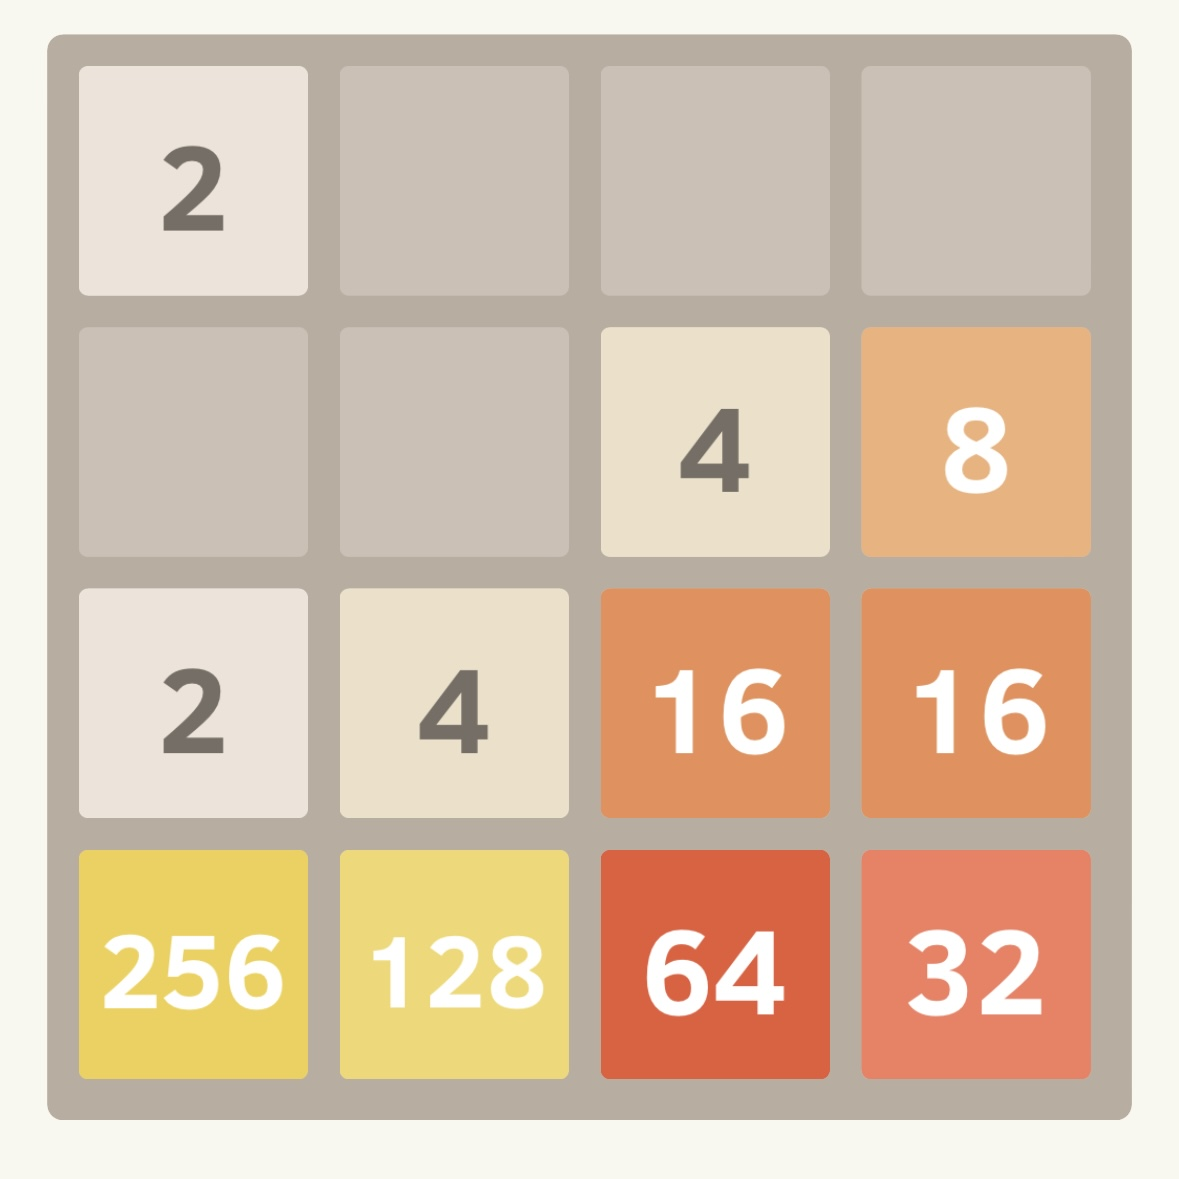
\includegraphics[scale=.05]{images/grid.jpg}
    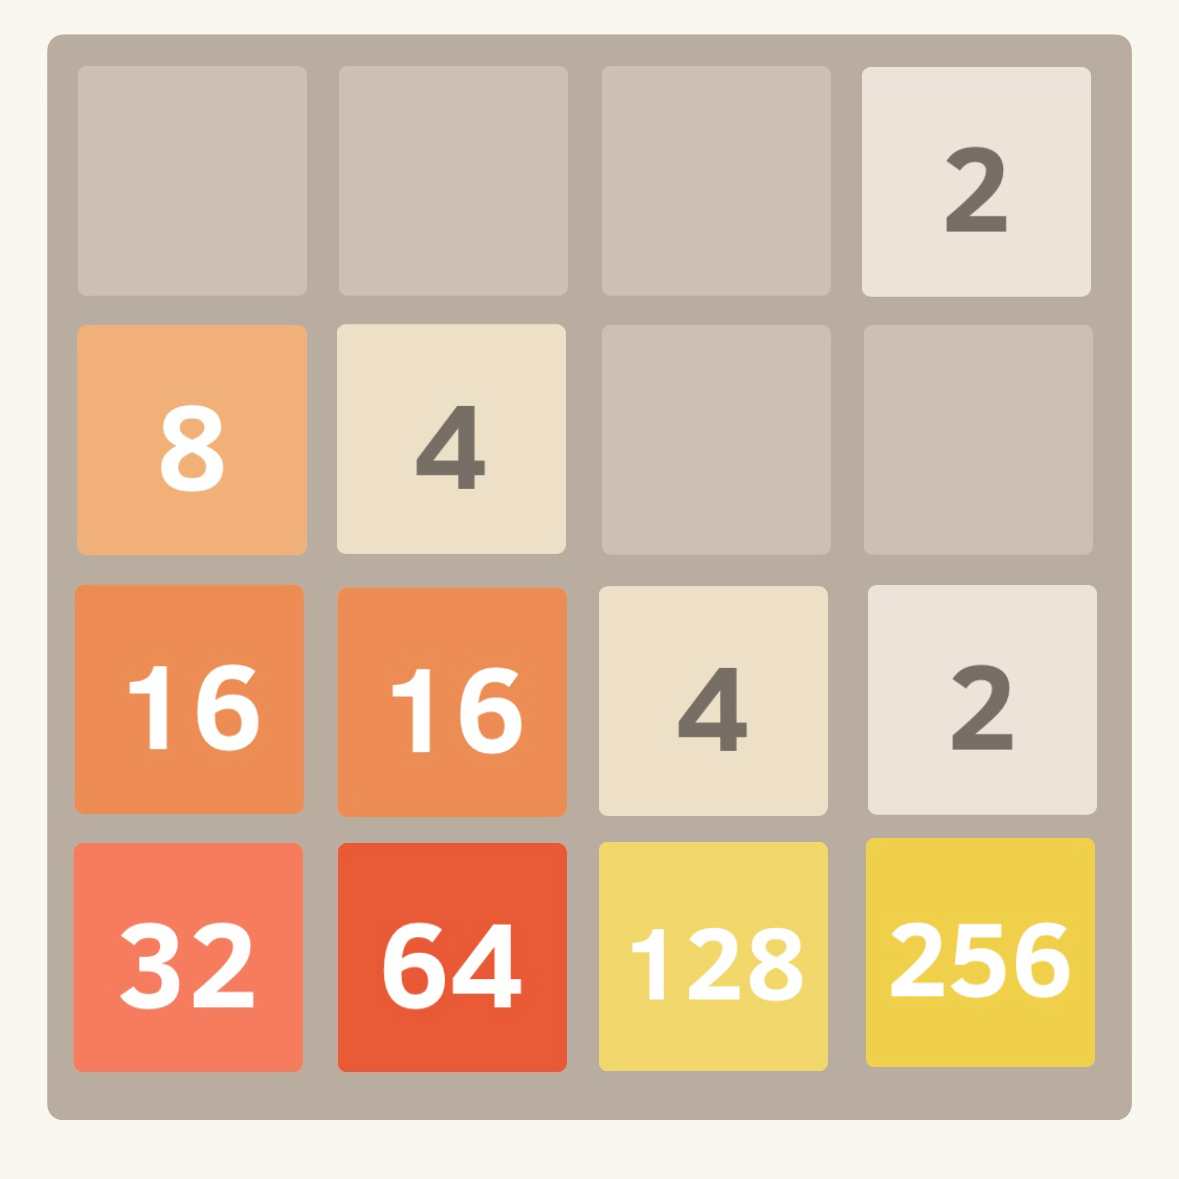
\includegraphics[scale=.05]{images/grid-reflect.jpg}
\end{center}

\subsection{Action}

\begin{center}
    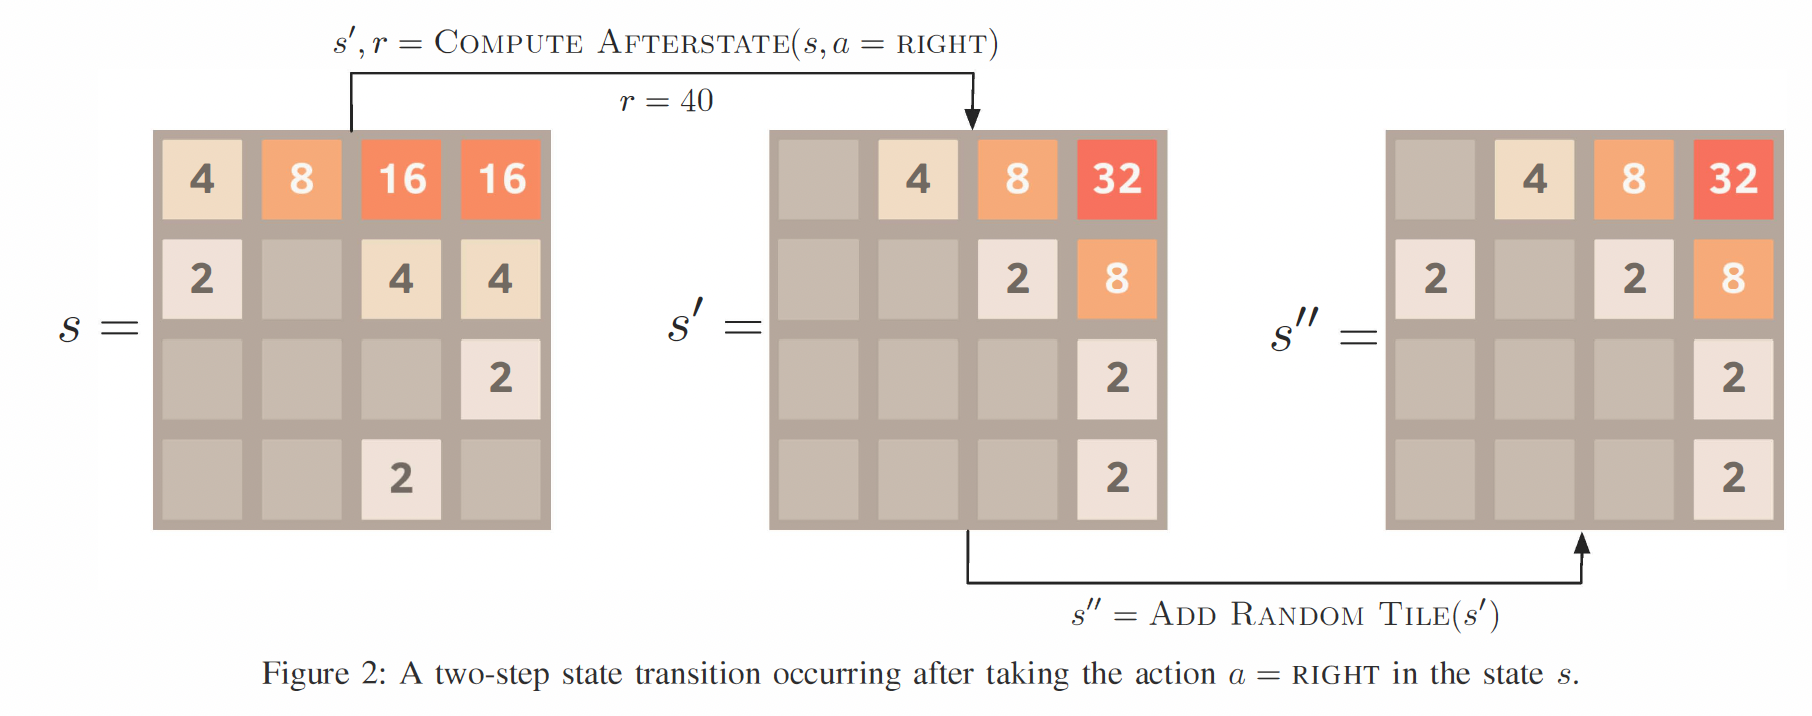
\includegraphics[scale=.25]{images/afterstate.png}
\end{center}

There are only for actions that correspond with sliding all tiles left, right, up or down: $A=\{L, R, U, D\}$. During the sliding of the tiles all same-value pairs closest to the direction of the slide get merged. A valid move is if the board changes after the move. After a valid move another additional tile spawns in a randomly chosen empty cell. The game ends when the board runs out of empty tiles and there are no legal moves to make.

An important distinction has to be made in the state transition process. There are two parts:
\begin{enumerate}
    \item a deterministic step that only slides and merges tiles in the direction of the action, an \textit{after-state} 
    \item a stochastic step that spawns a new tile, a \textit{next state}
\end{enumerate}
One can create a list of all possible transitions and their probabilities which means that this game can be modelled as a Markov Decision Process.


\subsection{Reward}

For this project we are going to use the reward that is provided by the environment. The reward is equal to the sum of all numbers of the merged tiles. For example, if an action results in a merge of two 2-tiles and two 8-tiles, reward $=(2 + 2) + (8 + 8) = 20$

\subsection{Simulator}


I used \href{https://pypi.org/project/gym-2048/}{gym} implementation of 2048 and added a few modifications in this \href{https://github.com/h0rban/gym-2048}{pull request}. I had to fix bugs, adjust the state to be represented as powers of 2, added the render function and useful helper functions.


\section{Methods}

\subsection{$n$-Tuple Networks}

\begin{center}
    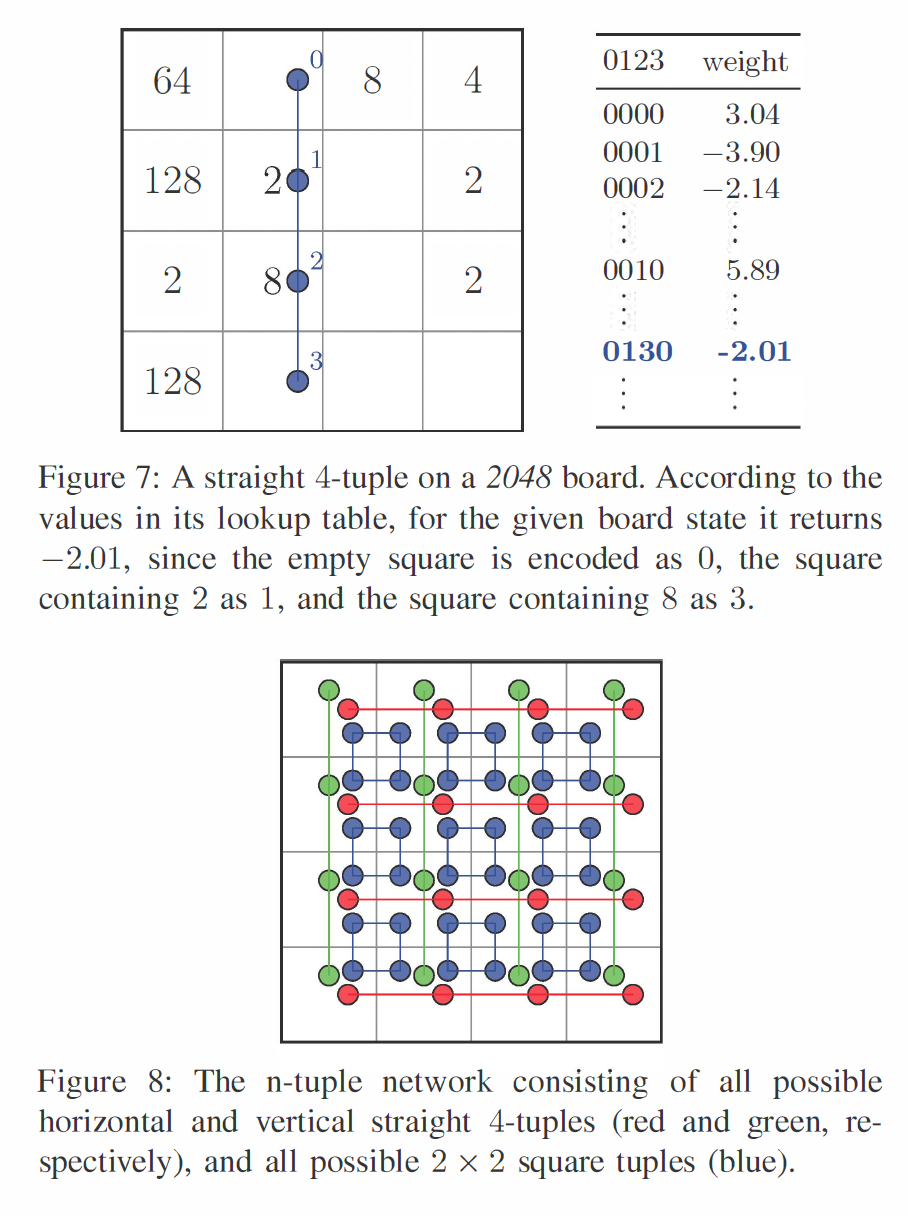
\includegraphics[scale=.5]{images/ntuple-network.png}
\end{center}

\begin{center}
    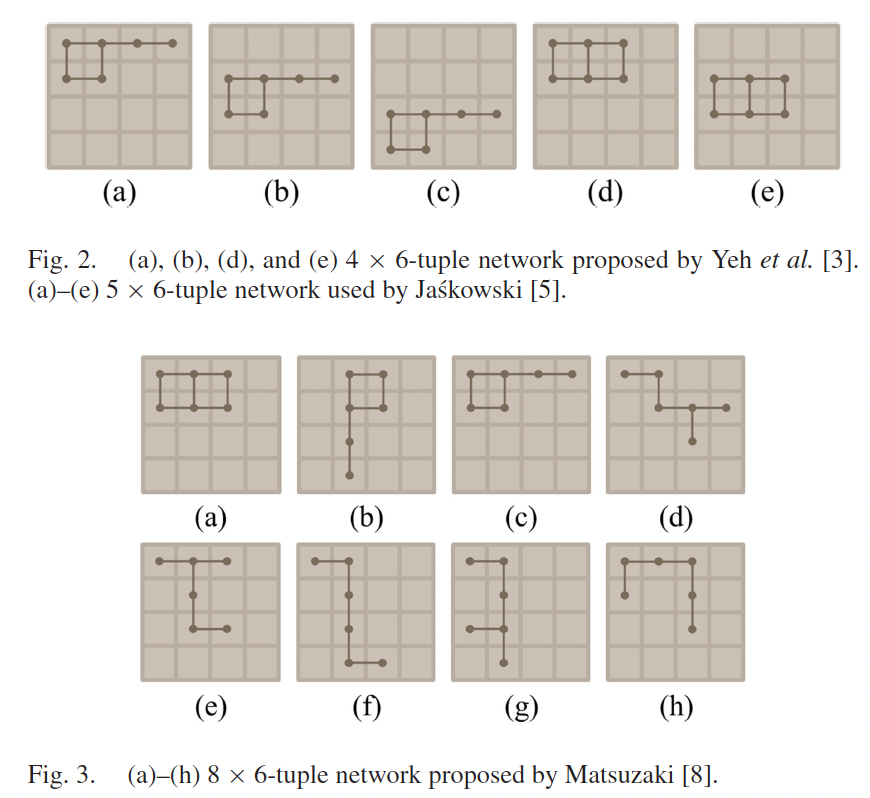
\includegraphics[scale=.5]{images/ntuple-network2.png}
\end{center}

\begin{align}
    V(s) = \sum_{i=1}^{m} LUT_i[\phi_i(s)]
\end{align}

Estimating the state value on the whole state is impractical so instead a N-Tuple Network function approximator is applied. Based on the cells of the $n$-tuple we construct a a set of feature weights and stored and updated it in a look up table. The state value estimation is then calculated by retrieving the feature vector and summing the weights.

I have followed the example of M. Szubert and W. Jaskowski with constructing a 4-tuple with the maximum tile value of $2^{15}=32678$ to limit the number of weights in the network. Similar to Figure 8, I have used 4 horizontal and vertical tuples, and 9 square tuples which resulted in $17 \times 15^4 = 860,625$ weights.


\subsection{Multi-stage TD Learning}

\begin{center}
    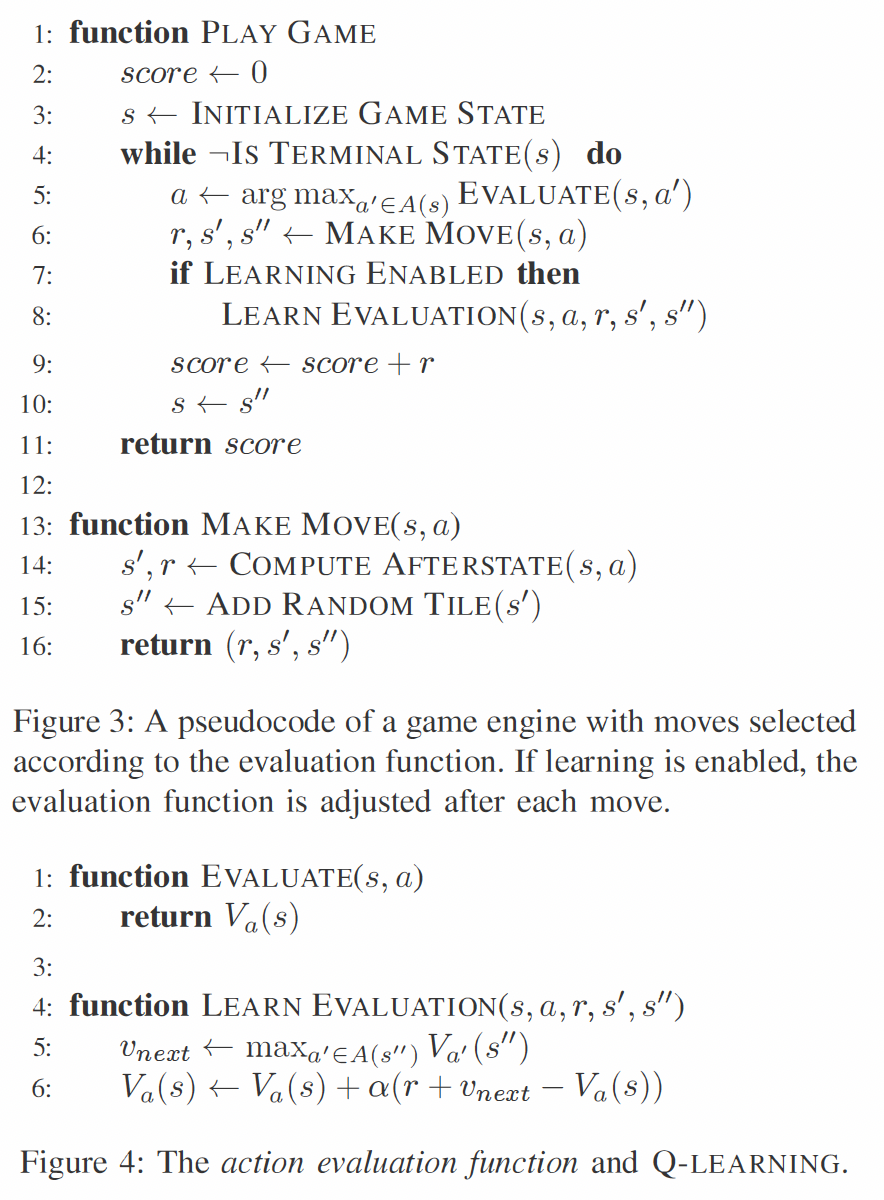
\includegraphics[scale=.5]{images/main-algo.png}
\end{center}

TD learning is intrinsically to train and learn to obtain average (or expected) scores as high as possible based on adjusting state values from the subsequent evaluations. However, research has shown that it preforms poorly on this task. Instead, we can use multi-stage TD learning, where the learning process is divided  into multiple stages, each of which has its own learning agent and sub-goal, e.g., reaching 8192-tiles or 16384-tiles.

\subsection{Optimistic Initialization}

Some works have shown that exploration techniques, such as $\epsilon$-greedy and softmax were not successful for this environment because it is not likely that an agent selects an unexplored state or action when revisiting it. Instead, we want to use Optimistic Initialization, so that large initial state value are reduced once the corresponding states are visited until all the actions are sufficiently explored.

\subsection{TC Learning}

\begin{align}
    \delta_t = r_{t+1} + V(s'_{t+1}) - V(s'_t)
\end{align}

TC learning is a TD variant with adaptive learning rates. Instead of adjusting the learning rate α directly, this method introduces new parameters weights $\beta$, $E$ and $A$.

\begin{align}
    \theta_i \gets \theta_i + \alpha \beta_i \delta_t
\end{align}

\begin{align}
    \beta_i = \begin{cases}
        |E_i| / A_i \text{ , if } A_i \neq 0\\
        1 \text{ , otherwise}
    \end{cases}
\end{align}

$\beta_i$ represents the coherence of $\theta_i$, and is calculated from two parameters $E_i$ and $A_i$ for each weight. Both $E_i$ and $A_i$ are initialized with 0 and adjusted by

\begin{align}
    E_i \gets E_i + \delta_t \text{ and } A_i \gets A_i + | \delta_t |
\end{align}

It is an effective method for this problem because it reduces weight adjustments to automatically accelerate network convergence, however it introduces a triple memory overhead.

\subsection{Expectimax Search}

\begin{center}
    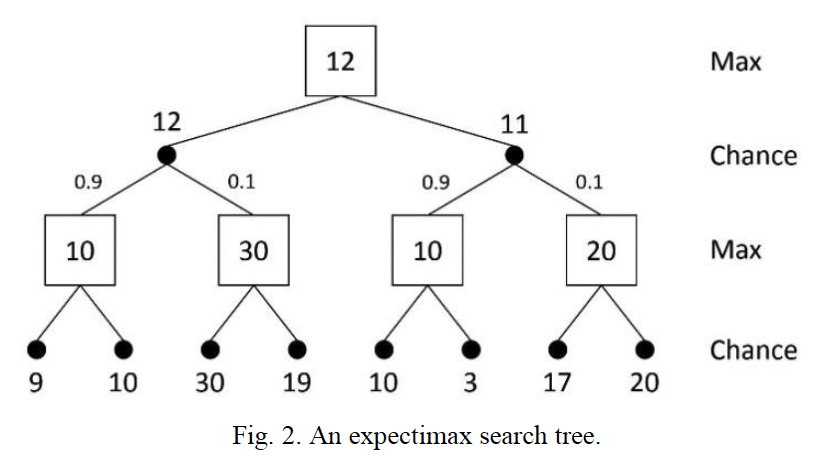
\includegraphics[scale=.5]{images/tree-search.png}
\end{center}

Like in most games, the search tree looks as the max node and the expected value of its children. Features used for Expectimax Search are monotonicity of a board, number of empty tiles, number of mergeable tiles, but there can be more.

To speed up the search we should use the Transposition Table to avoid searching redundant states. Common implementation is a Zorbist hashing algorithm based on doing an exclusive or operation on the 16 keys of the grid cells. As described in the state section, we can also include board reflections to reduce the number of leaves needed to search.

The board is considered to have high \textit{monotonicity} if the values are either non-increasing along all rows or non-decreasing along all rows and if the values are non-increasing along all columns or non-increasing along all columns, with the highest value being in one of the four corners. Algorithm 2 describes a simplified version of the process used to score a single game state’s monotonicity. Rotating 90 degrees clockwise is to transform all coordinates such that such that 
\begin{align}
    G_r [3 - y][x] \gets G[x][y]
\end{align}
for all x and y. In the code, the board is only rotated once, with two corners being checked per rotation (the second corner is checked by substituting the $\geq$ on lines 7 and 14 with $\leq$).

\begin{center}
    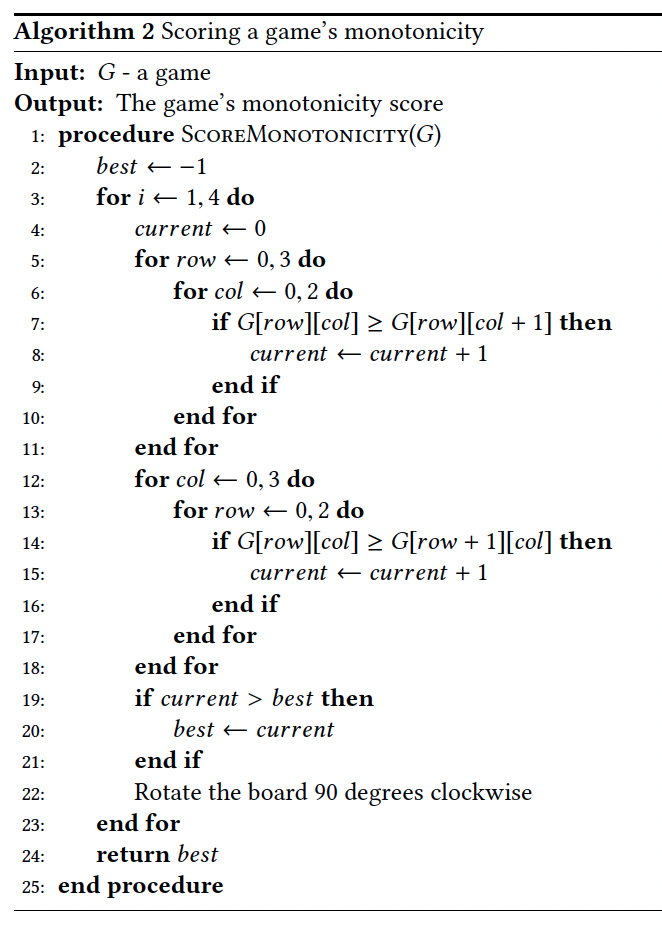
\includegraphics[scale=.7]{images/monotonicity.png}
\end{center}

\section{Results}

\begin{center}
    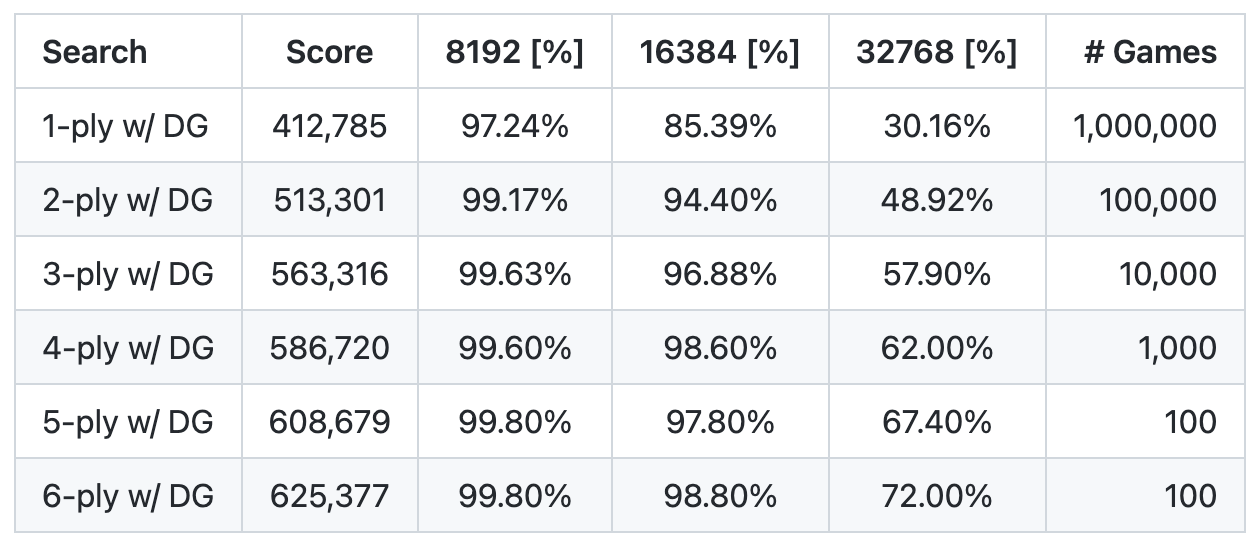
\includegraphics[scale=.4]{images/result-table.png}
\end{center}

In addition, for sufficiently large tests, 65536-tiles are reached at a rate of 0.02\%.

The results above are from \href{https://github.com/moporgic/TDL2048}{https://github.com/moporgic/TDL2048}, a state of the art optimistic TD+TC (OTD+TC) learning for training and tile-downgrading (DG) expectimax search for testing. 

As described in the multi-stage TD learning section, avarage total score or number of steps in the game are not necesarily the best metric for evaluating the algorithms. Instead we want to look at the rate at which the high-valued tiles are reached. One can notice that if we increase the depth of the search tree ($n$-ply) then we get consistently better results, but it becomes more computationally expensive to run simulations so the number of games in the table is smaller.

\begin{center}
    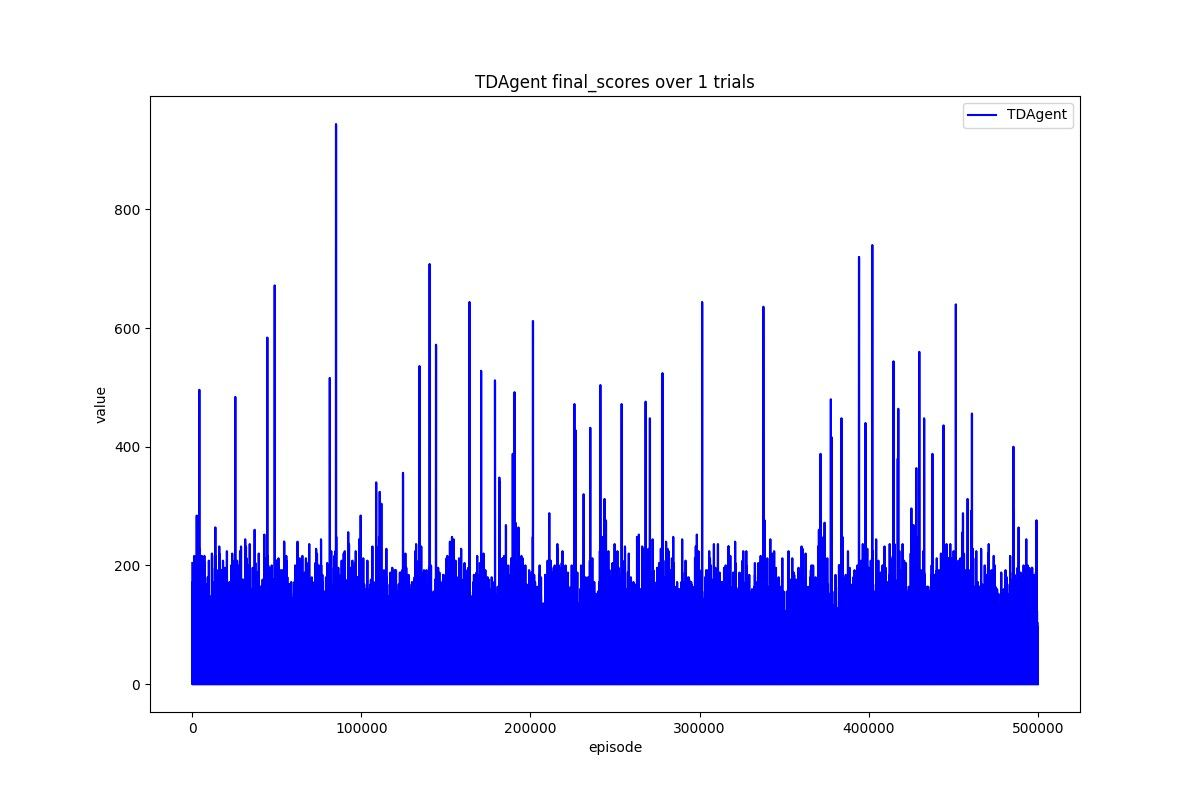
\includegraphics[scale=.2]{images/results.jpg}
\end{center}

My results in the graph above show that my agent is not improving over 500K trials, which suggests that I have a bug in my implementation.


\section{Future work}

So far, I only implemented a regular TD Learning algorithm with 17 4-tuple networks. Firstly, I want to find a bug that prevents my agent from learning and add additional learning methods described in this paper. MSTD might be the next easiest method to implement.

With a more successful implementation I want to:
\begin{enumerate}
    \item check if the algorithm uses the corner for the highest tile and cascades the smaller tiles in a ladder pattern
    \item check if the algorithm risks to bring the highest tile back into the corner in case it was forced out of it
    \item how often the algorithm looses the game as the result of a forced move - for example when you are collecting a high valued tile in the bottom left and need to make an "up" action that ruins the tile chain
\end{enumerate}

\bibliography{aaai22}

\bibentry{otd}
\bibentry{cbh}
\bibentry{mstd}
\bibentry{tdnn}

\section{Appendix}

Code \href{https://github.com/h0rban/2048-rl}{https://github.com/h0rban/2048-rl}

\noindent
Lecture slides \href{https://docs.google.com/presentation/d/1lhgJfJ3f-rJLfIHltV4ai3gLgtf5U6HSHPXfUvBGsnk/edit?usp=sharing}{https://docs.google.com/presentation/d/1lhgJfJ3f-rJLfIHltV4ai3gLgtf5U6HSHPXfUvBGsnk/edit?usp=sharing}

\end{document}
